\chapter{Liste des théologiens}
% ToC of the main sections
\startcontents[mainsections]
\printcontents[mainsections]{l}{1}{\section*{Liste des théologiens et islamologues}\setcounter{tocdepth}{4}}
 


%------------------------------------------------------------
\section{Philosophes des Lumières}
%------------------------------------------------------------
\paragraph{Al Kindi}  \mn{\cite{PolDroit:voyage}  (p. 277).   }

Le premier d’entre eux, Al-Kindî (né vers 800, mort vers 870), est ainsi l’auteur d’une œuvre encyclopédique, qui aurait compris plus de deux cents titres, dont un cinquième environ nous est parvenu, où se juxtaposent traités de géométrie et de physique, de pharmacopée et de chiffrement des messages. Dans son Livre de la philosophie première, dont il ne reste que la première partie, il définit la philosophie, dans le droit fil d’Aristote, comme « la science des choses en leur vérité autant que
l’homme en est capable ». Or, puisque la vérité est une, elle ne saurait différer selon qu’on y parvient par la raison ou par la révélation. En suivant la voie de la rationalité, la philosophie ne peut contredire ce qu’enseignent les prophètes au sujet de la vertu. Si différence il y a, comme l’explique Al-Kindî dans son Épître sur le nombre des livres d’Aristote, elle ne tient qu’à des modalités distinctes dans la voie d’accès au vrai. La science philosophique est humaine et acquise par des moyens humains. Elle s’obtient au prix de longs efforts, s’exprime au moyen d’explications et de processus graduels. La science divine, au contraire, se communique aux prophètes intégralement, d’un seul coup, de manière lapidaire. Voilà pourquoi il faut parfois des pages et des pages pour commenter seulement un verset du Coran. Mais, entre philosophie et prophétie, seuls les chemins s’opposent. Les buts visés, comme les réalités atteintes, sont identiques. Il serait trop simple de croire qu’Al-Kindî, et à sa suite les grands représentants de la falsafa, se bornent à proclamer l’absence de contradiction
entre le cheminement pas à pas de la raison et la fulgurance de la révélation prophétique. Ils entament également un travail de reformulation, de réélaboration des concepts grecs et de leurs relations internes. Ainsi, par exemple, Al-Kindî transforme-t-il profondément la conception de l’action que développe Aristote pour faire de la création la forme première de l’action et parvenir à concevoir en termes grecs une réalité révélée qui leur était opposée : la création du monde par Dieu. Les concepts semblent les mêmes, leur sens ne l’est plus. Plutôt qu’un simple héritage, plutôt qu’une filiation, il s’agit bien d’une reconstruction, d’une création qui ouvre peu à peu la voie à des perspectives philosophiques nouvelles, et fort différentes de celles des Grecs.


%------------------------------------------------------------
\paragraph{Al Farabi} \mn{\cite{PolDroit:voyage}  (p. 278).   }  
Al-Fârâbî naît en 872, dans l’actuel Kazakhstan, étudie à Bagdad, et meurt à Damas, en Syrie, en 950. Lui aussi s’efforce de concilier Platon et Aristote, qu’il considère comme les deux auteurs d’une seule et même sagesse, et pose une série de nouveaux jalons décisifs pour le développement
ultérieur de la falsafa. À côté de multiples travaux de mathématiques et d’optique, d’un Grand livre de musique (c’était un bon joueur de luth) et d’une critique de la médecine, qu’il rabaisse au rang d’une routine empirique, Al-Fârâbî est le premier à souligner le rôle central de la notion d’« intellect agent », qui va occuper une place prépondérante chez ses successeurs et, plus tard encore, chez les lecteurs chrétiens des philosophes arabo-musulmans. On doit enfin à la sagacité d’Al-Fârâbî d’avoir mis en lumière les stratégies politiques envisageables dans différents types de Cité. Selon que la Cité est « vertueuse » ou « ignorante », qu’elle dispose du strict « nécessaire » ou de la prospérité de l’« échange », selon qu’elle vise « la gloire » ou bien « la puissance », selon qu’elle est « versatile » (ses idées ne cessent de changer) ou « égarée » (elle veut le bien mais se trompe de bien), elle a besoin d’un style de gouvernance différent. Dans ce domaine, Al-Fârâbî s’inspire de Platon, mais va dans une tout autre direction, ouvrant la voie à une réflexion politique pragmatiste très en avance sur son temps.Son rôle est donc crucial, car Al-Fârâbî renforce l’attention à porter à la logique et la métaphysique grecques, relit et prolonge Platon, en le fusionnant avec Aristote, considéré comme le « premier maître » de tous les philosophes. Maïmonide n’hésitera pas à surnommer Al-Fârâbî « le second maître ».


\paragraph{l'intellect humain}
Elle vient d'Aristote qui discerne dans l'intelligence (le \textit{nous} l'esprit qui distingue), une réception passive des informations (intellect passif) présente dans chaque être humain, et d'autre part une activité d'élaboration des formes et des vérités éternelles. Les hommes n'ont pas la possibilité de les former mais uniquement de les atteindre. Mais Les philosophes arabes vont lire cela différemment d'Aristote, et comprennent la notion d'intellect gent comme une sorte d'intelligence divine collective : l'homme qui accède à une vérité (en faisant une démonstration, en calculant,...) n'y parvient pas par lui-même et de manière isolée, mais en participant, le temps de son intellection, à l'intellect divin. Cette conception a donné lieu à des débats très nombreux et complexes, et les conflits d’interprétation abondent. Mais la portée et les conséquences de cette idée d’intellect agent sont grandes, et simples à entrevoir : si l’homme qui exerce sa réflexion pour atteindre une vérité participe à un processus de compréhension qui le dépasse entièrement, s’il se connecte, même sans le savoir, à l’intelligence divine chaque fois qu’il calcule, voilà qui, de proche en proche, vient troubler gravement les frontières entre subjectif et objectif, individuel et collectif, humain et divin, philosophique et religieux... En effet, il ne saurait plus être question d'opinion personnlle mais d'intelligence conforme, ni de tâtonnement humain mais d'intellection vraie. et la philosophie comme travail imparfait de l'intelligence humaine devient découverte des vérités divine par participation, directe ou intdirecte, à l'intelligence divine. \sn{\cite{PolDroit:voyage} p.280}
 
\begin{Synthesis}[Actualité de l'intellect Humain]
  il est curieux que l'intellect Humaine ne soit pas reconsidéré aujourd’hui avec d’autres yeux. Dans la participation permanente de chacun au monde numérisé, connecté, dominé par l’intelligence artificielle et l’intelligence collective, est-on sûr que les anciennes spéculations sur l’intellect agent n’auraient rien à nous dire ? \sn{\cite{PolDroit:voyage}, p 280}
 
\end{Synthesis}

 
%------------------------------------------------------------
\paragraph{Avicenne}




%------------------------------------------------------------
\subsection{al-Ġazālī}

le joyau d'al-Ġazālī~: \emph{Le Tabernacle des Lumières}, traduit
par Deladrière, Paris, Seuil, texte très dense et très profond aux
implications nombreuses.
\paragraph{Al-Ghazâlî, l’anti-philosophe} 
\begin{quote}
Les philosophes se trompent. La raison ne peut conduire aux vérités divines. Seuls les prophètes les connaissent et montrent le chemin. La révélation étant la seule voie de salut, les philosophes sont néfastes, et même condamnables,s’ils en détournent. Il convient donc de les combattre, au nom de la religion, qu’ils menacent. Tel est, en substance, le contenu d’un traité que publie en 1095 Al-Ghazâlî. Son titre est explicite et polémique : L’Incohérence des philosophes (Tahâfut al-Falâsifa). Le terme arabe Tahâfut signifie à la fois « bavardage », « non-sens » et « excès ». Selon Al-Ghazâlî, les philosophes parlent pour ne rien dire, tiennent des discours contradictoires, ont des prétentions indues. Pour ce défenseur ardent de la religion contre le danger que constituerait envers elle la philosophie, mieux vaut lire le Coran que les œuvres d’Aristote. Il s’en prend en particulier à l’œuvre d’Avicenne, devenue de plus en plus influente. Écrivant à l’apogée de la falsafa, Al-Ghazâlî en souligne les limites, les difficultés et les points faibles. Sa défense et illustration de la révélation rencontrera une audience considérable, et Avicenne publiera une réfutation de sa réfutation des philosophes, en 1179, sous le titre L’Incohérence de l’incohérence. Ce débat historique peut à son tour se lire de deux manières différentes. On peut y voir la réaction des tenants de la prophétie et de sa primauté face à l’emprise grandissante de la philosophie. À ce titre, Al-Ghazâlî aura non seulement des admirateurs jusqu’à nos jours pour sa défense de la révélation, mais aussi des « imitateurs », si l’on ose dire, adoptant, dans leur domaine spirituel, une attitude analogue à la sienne. Ainsi Juda Halévi combat-il les philosophes juifs au nom de la Loi de Moïse, et Thomas d’Aquin, qui a lu Al-Ghazâlî de près, se garde-t-il de faire simplement de la philosophie la voie d’accès à Dieu. Dans cette lecture, il s’agit uniquement de prendre parti pour la révélation, contre la raison. Mais on peut aussi lire Al-Ghazâlî autrement. Comme un philosophe, tout autant qu’un adversaire de la philosophie. Car cet apologiste de la révélation et de l’expérience mystique est aussi, comme Pascal, un remarquable artisan des concepts. Sa critique des philosophes puise dans leurs œuvres, se nourrit de leurs démarches, utilise leurs outils – pour les retourner contre eux.Au lieu de considérer, trop simplement, que cette querelle opposerait ceux qui sont « dans » la philosophie et ceux qui se tiennent « au-dehors », mieux vaudrait l’envisager comme \emph{un conflit interne au registre philosophique.}
\sn{\cite{PolDroit:voyage}, p. 284}
 

 
\end{quote}
\cpageref{theol:AlGazali1,theol:AlGazali4,theol:AlGazali5,theol:AlGazali6,theol:AlGazali7,theol:AlGazali9,theol:AlGazali10,theol:AlGazali11,theol:AlGazali13,theol:AlGazali14,theol:AlGazali16,theol:AlGazali17,theol:AlGazali18,theol:AlGazali19,theol:AlGazali20,theol:AlGazali21,theol:AlGazali22,theol:AlGazali23,theol:AlGazali24}
\pageref{theol:AlGazali29}
\pageref{theol:AlGazali2}
\pageref{theol:AlGazali3}
\pageref{theol:AlGazali8}
%\pageref{theol:AlGazali31}
\pageref{theol:AlGazali25}
%theol:AlGazali31,theol:AlGazali32,theol:AlGazali33,theol:AlGazali34,theol:AlGazali35,theol:AlGazali36,theol:AlGazali37,theol:AlGazali38} 
%\label{theol:AlGazali1}



\section{Autres Théologiens Classiques Musulmans}
%------------------------------------------------------------
\subsection{Ibn Taymiyya}


 

C'est le très grand penseur (controversé) du 13\textsuperscript{ème}
siècle. Un certain nombre de ses ouvrages ont été traduits (souvent mal,
je sélectionne les meilleures traductions).


\emph{La lettre de Palmyre} traite de deux questions théologiques~: les
attributs divins et la prédestination~!

%\includegraphics[width=0.3\textwidth]{Images/image26.png}
\begin{marginfigure}
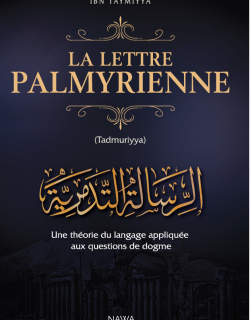
\includegraphics[width=0.5\textwidth]{Images/image026.png}
\end{marginfigure}

-~Ibn Taymiyya, \emph{Réponse Raisonnable aux Chretiens ?} édité,
traduit et commenté par Laurent Basanese, sj., Ifpo, 2011.

-~Ibn Taymiyya, \emph{Musique et danse selon Ibn Taymiyya}: Le livre du
\emph{Samâ°} et de la danse (\emph{Kitâb al-Samâ° wa l-Raq.s}), Paris,
Vrin, 2000.

-~Ibn Taymiyya, \emph{Pourquoi les savants divergent,} Al-Hadith
éditions, 2012


Voir p. \pageref{ibn-taymiyya}.


%------------------------------------------------------------
\subsection{Ibn Toumart}
\label{IbnToumart}
\mn{E.B., « Ibn Toumart », in 23 | Hiempsal – Icosium, Aix-en-Provence, Edisud (« Volumes »,
no 23) , 2000 \url{http://encyclopedieberbere.revues.org/1629}}


Ibn Toumart est la personnalité religieuse et politique la plus marquante du Maghreb au
XIIe siècle. Fondateur du mouvement almohade*, il devait préparer la revanche des Sanhadja
montagnards contre l’empire déjà vacillant des Almoravides. Bien que ses disciples aient
manipulé sans vergogne sa généalogie pour le rattacher à la descendance du Prophète et en
faire, donc, un chérif, il est sûr qu’Ibn Toumart était issu d’une tribu du Sous, celle des Hergha,
appartenant au groupe montagnard des Maçmouda.
 L’un de ses premiers disciples, le pieux el Baïdaq, se fit son chroniqueur et grâce à son
récit, souvent dithyrambique, il est possible de saisir l’évolution spirituelle de celui qui
devait mériter le titre de Mahdi Almohade et le qualificatif d’Impeccable. Célèbre dès son
adolescence, pour son zèle religieux et son érudition qui lui avait fait donner le surnom d’asufu
(le tison, le flambeau, en berbère), Ibn Toumart quitta un beau jour son village d’Igliz et
ses montagnes pour compléter, en Orient, sa connaissance de l’islam et jeter les bases d’une
réforme radicale.
 Son séjour en Espagne n’est pas assuré, mais demeurent des concordances étroites entre
les textes d’Ibn Hazm et ses propres propositions. En revanche, sa présence à Bagdad est
pleinement confirmée, alors que son passage à Damas est peut-être légendaire et les entretiens
qu’on lui prête avec Ghazali certainement inventés.
 Dix ans après son départ d’Igliz, Ibn Toumart entreprend un long voyage de retour au Maghreb,
au cours duquel il multiplie les étapes, passant par Alexandrie, Tripoli, Mahdia, Tunis,
Constantine et Béjaia. Sa condamnation des moeurs citadines relâchées provoque souvent des
échauffourées. A Béjaia, ses violences verbales déclenchent la fureur populaire contre lui. Le
sultan hammadite, qui l’avait d’abord bien accueilli, lança ses sicaires à sa poursuite, mais Ibn
Toumart trouva refuge dans la tribu voisine, celle des Beni Urigol, dans le village de Melala.
\paragraph{
La doctrine almohade}
 Ibn Toumart y élabore sa doctrine et réunit ses premiers disciples. Le plus cher à son coeur,
celui qu’il considère comme l’homme providentiel qui doit lui succéder, est Abd el Moumen,
le fils d’un potier de Nédroma (Algérie occidentale). El Baïdaq nous a laissé le récit émouvant
de la désignation du futur calife. Le réformateur proclama un soir en prenant sa main : “La
mission sur laquelle repose la vie de la religion ne triomphera que par Abd el Moumen ben Ali,
le flambeau des Almohades.” Celui-ci, en pleurant, dit avec humilité : “Ô Maître, je n’étais
nullement qualifié pour ce rôle, je ne suis qu’un homme qui cherche ce qui pourra effacer ses
péchés.” – “Ce qui te purifiera de tes péchés, répondit Ibn Toumart, ce sera précisément le rôle
que tu joueras dans la réforme de ce monde.”
 Une conversation avec deux pèlerins de l’Atlas qui passaient par Bougie est l’occasion du
départ des premiers Almohades vers le Maghreb el Aqsa. La petite troupe, d’une dizaine de
personnes, gagne Marrakech non sans avoir semé la bonne parole et causé quelques troubles
dans les villes traversées : Tlemcen, Oujda, Taza, Fès, où Ibn Toumart se fait remarquer par
le saccage des magasins des marchands de musique, contre lesquels il semble avoir eu une
aversion certaine. Il réitère à Marrakech, brisant à coups de bâton instruments de musique
et jarres de vin, pourchassant sous les huées la soeur de l’émir almoravide, qui chevauchait
dévoilée dans les rues de la capitale.
 Après la prise de Tin Mel (1123), il se proclame Mahdi et, de retour dans les tribus Masmouda,
ses frères de race, il organise solidement la communauté almohade avec un soin et une
connaissance des hommes qui font de ce clerc un grand homme d’État. Il crée un véritable
État montagnard, solidement organisé, disposant d’une armée fanatisée chargée de répandre
la doctrine almohade jusqu’en Ifriqiya et en Espagne.

Nous retrouvons dans cette réforme la même tendance innée vers le rigorisme moral et la
simplicité doctrinale que nous ont révélés tous les schismes et hérésies nés en Berbérie à travers
les siècles.
Dans la condamnation absolue des richesses de ce monde et de ses frivolités, c’est la voix
d’Ibn Toumart qui tonne, mais elle fait écho à celle, non moins véhémente, de Tertullien. La
lente marche des Berbères vers le Dieu unique semble ici se parachever dans la proclamation
de l’Unicité absolue de Dieu, dont Ibn Toumart rejette jusqu’aux adjectifs (le Puissant,
le Miséricordieux, le Victorieux) que lui dorment les musulmans, parce qu’ils risquent de
faire apparaître comme divisible la puissance divine. La conséquence inévitable de la toute puissance
de Dieu ainsi comprise est la prédestination de tous les êtres créés : chacun doit
attendre dans la soumission totale ce qui lui a été assigné de toute éternité.
Cette forme de l’islam ne peut qu’être fanatique, elle ne supporte ni relâchement des moeurs,
ni relativisme dans le dogme, ni présence d’Infidèles.
11 Ces données concordaient trop bien avec l’intransigeance fondamentale des Berbères pour ne
pas aboutir : aussi, sous Abd el Moumen, le raz de marée almohade balaya le Maghreb de
toute impureté. C’est alors, semble-t-il, que disparurent les dernières communautés chrétiennes
autochtones.
\paragraph{L’État almohade}
Respectueux des traditions tribales des Berbères du Haut Atlas, Ibn Toumart organisa son
gouvernement en établissant une hiérarchie entre différents conseils imités des assemblées
tribales. Au sommet siège le Conseil des Dix, qui sont les premiers et les plus fidèles
compagnons (Abd el-Moumen*, Abou Hafs Omar*, El Bachir...). Au-dessous du Conseil
des Dix, le Conseil des Cinquante est composé de contribules d’Ibn Toumart, des Hergha et
d’autres Maçmouda de Tin Mel ou des Hintata. Les différentes tribus de la montagne étaient
ainsi représentées dans ce Conseil dont les pouvoirs étaient restreints.
Toute la société almohade était strictement hiérarchisée. A l’intérieur des groupements
ethniques apparaissait une autre hiérarchie, fondée sur les fonctions exercées, depuis celles
des compagnons les plus proches jusqu’à celles confiées aux abid (serviteurs noirs). Au
sommet de la pyramide, le Mahdi tenait solidement les rênes d’un pouvoir absolu. Cette
domination reposait sur une logique implacable : tout Almohade suspecté de tiédeur risquait
l’élimination : ainsi lors de la “journée du tri” plusieurs milliers d’almohades “infidèles” furent
massacrés. C’est par de telles actions qu’Ibn Toumart réussit à construire l’État almohade et à
assurer la naissance de la nouvelle dynastie moumenide. Seuls le prestige et la volonté d’Ibn
Toumart réussirent à faire admettre Abd el-Moumen comme le successeur désigné du Mahdi.
Encore fut-il nécessaire de cacher la mort de celui-ci pendant plus de deux ans avant de faire
reconnaître le nouveau souverain par les Cheikhs almohades.
\paragraph{références}
voir p. \cpageref{theol:IbnTumart1}


%------------------------------------------------------------
\subsection{Autres théologiens classiques}

%------------------------------------------------------------
\paragraph{Ibn Hanbal}

voir p. \pageref{Theol:IbnHanbal1}


 \paragraph{Ibn Hazm} \label{Theol:IbnHazm}{Ibn Hazm est un théologien andalou de Cordoue mort en 456H / 1064 dont
la famille s'était convertie à l'islam quelques deux siècles auparavant.
Il est à la fois poète, théologien, philosophe, historien. Son œuvre
comprend près de 400 ouvrages dont le fameux \emph{Collier de la colombe
sur l'amour et les amants}, où il aborde sous forme d'anecdotes les
manifestations et signes de l'amour. Ses analyses psychologiques sont
d'une grande finesse et s'appuient sur une perspective platonicienne où
l'amour est vu comme union des âmes à la lumière du principe de la
ressemblance. En droit, c'est un ẓahirite (extérioriste, littéraliste).
Il est très méfiant à l'égard de l'utilisation de l'analogie ou de
l'opinion~: pour lui, on doit respecter le texte dans sa littéralité. Il
a rédigé un \emph{Traité sur les religions et les écoles de pensée}. }

voir p. \pageref{Theol:IbnHazm1}, \pageref{Theol:IbnHazm2} - Polémique de Ratisbonne avec Benoit XVI.
%------------------------------------------------------------
\paragraph{Ibn Salah}
Ibn Salah
\pageref{Ibnsalah1}
%------------------------------------------------------------
\paragraph{Ibn Khaldūn} \label{Theol:IbnKhaldun} penseur andalou Ibn Khaldūn p. \pageref{theol:IbnKhaldun}, \pageref{Theol:IbnKhaldun2}
%------------------------------------------------------------
\paragraph{Ibn Qutayba}
Ibn Qutayba -- si ce nom ne vous est pas encore familier, cela devrait
faire `tilt' car nous l'avons rencontré au début de cette leçon. Il a
écrit un Traité sur comment rendre compte et comprendre les divergences
dans le \emph{ḥadīṯ.} A-t-il été traduit en français~? La réponse est en
note 3 --
\pageref{Theol:IbnQutayba1}
%------------------------------------------------------------
\paragraph{Kalābāḏī}
  est un auteur persan, mort aux environs de 990. Cet ouvrage
cherche à réconcilier le soufisme et l'orthodoxie. 
\pageref{theol:Kalabadi}


\paragraph{Ibn 'Arabi} Soufi, voir p. \pageref{Theo:IbnArabi}.




%------------------------------------------------------------
\section{Théologiens modernes}

%-------------------------------------------------
%------------------------------------------------------------
\paragraph{ʿAlī Ṭanṭāwī} \label{theo:AliAlTawani}
{Ali Al tantawi est originaire d'une
famille de lettrés égyptiens qui a émigré à Damas à la fin du XIXème
siècle.


Il s'est opposé à l'impérialisme occidental dans les pays
arabes et, en particulier, à la présence de la France comme mandataire
en Syrie et celle de l'Angleterre en Irak. Après l'indépendance de la
Syrie, en 1947, ses positions contre le communisme, qu'il considère
incompatible avec l'Islam lui valent d'être menacé dans son propre pays.
En 1963, il quitte la Syrie pour l'Arabie Saoudite et devient
enseignant.
Extrêmement populaire dans son pays d'adoption, il a
présenté des programmes à la radio et à la télévision pendant un quart
de
siècle.}

%-------------------------------------------------------
\label{theol:SayyidQutb}
\paragraph{Sayyid Qutb}
Sayyid Qutb (arabe :\TArabe{ سيد قطب,} Sayyid Quṭb), né le 9 octobre 1906, dans le sud de l'Égypte, et exécuté par pendaison le 29 août 1966 au Caire, est un poète, essayiste et critique littéraire égyptien, puis un militant musulman membre des Frères musulmans. Il entrera en rupture avec ces derniers à la suite du développement d'une idéologie islamiste radicale, le \textbf{qutbisme}.


Les idées de Sayyid Qutb se résument schématiquement ainsi :
\begin{itemize}
    \item 
L'islam est en crise. Les millions de gens qui se réclament de l'islam n'en comprennent en réalité pas grand-chose, ils ne sont pas de vrais musulmans. Qutb prononce donc une condamnation très forte de la société égyptienne contemporaine.
  \item 
Un retour aux vraies valeurs de l'islam est nécessaire. Malheureusement les masses populaires manipulées par le nassérisme sont incapables de s’en sortir. Il appartient donc à une élite de guider les masses en jouant le même rôle que celui des compagnons du prophète de l'islam; cette élite qu'il appellera dans plus d'un ouvrage "\textit{annawâte assoulba}" (littéralement "le noyau dur"). Le but est de réislamiser la société.
  \item 
L'islam apporte une solution complète à tous les problèmes, politiques, économiques, sociaux. En revanche, les influences occidentales sont dangereuses et nuisibles. Il dénie le qualificatif de « civilisation » (notamment dans son livre Mushkilât al-hadâra : Problèmes de la civilisation) aux blocs de l'est (socialiste) et de l'ouest (capitaliste), qu'il renvoie dos à dos comme représentant deux faces d'une même entité qu'il qualifie de \textit{Jahiliya} (ignorance). Ce terme, qui renvoie à la période précédant l'islam durant laquelle l'Arabie était polythéiste et ignorante donc du vrai Dieu, a une forte connotation négative dans l'imaginaire musulman.
  \item 
L'idée d'une « lutte contre les Juifs » fut aussi présente dans la pensée de Sayyid Qutb, qui écrivit au début des années 1950 l'opuscule \textit{Notre combat contre les Juifs}. Dans son commentaire de la sourate 5, Sayyid Qutb réaffirmera l’accusation : « Depuis les premiers jours de l’islam, le monde musulman a toujours dû affronter des problèmes issus de complots juifs. (…) Leurs intrigues ont continué jusqu’à aujourd’hui et ils continuent à en ourdir de nouvelles. » 
\end{itemize}




%----------------------------------------------------------------------------------------------------
\section{les figures de l'Islam de France}
\label{sec:figuresIslamFrance}
\mn{\CB}
\subsection{Les pionniers }

Les premiers recteurs de la Grande mosquée de Paris :
\paragraph{Si Kaddour Benghabrit} (Sidi Bel Abbès 1868 – Paris 1954): Tendance malikite algérienne. Sa vie s’étend sur 3 pays; théologien et magistrat algérien, formé à la Qaraouiyine (Fès, Maroc), Fondateur de l’Institut Musulmans de la Grande mosquée de Paris, dont il fût le 1er recteur (détails dans le cours). Sous le protectorat, un statut d'interprète (cadre du MAE), avant la loi de 1905. Aidera le roi Hassan I à faire un certain nombre de réformes . Consul général honoraire à Fez. Le maréchal Lyautey l'envoie dans le Hijaz pour le Haj. Créera la société des Habous, à l'origine de la Grande mosquée de Paris (1926)

\paragraph{Si Hamza Boubakeur} (Brezina 1912 – Paris 1995): Tendance malikite algérienne. Cursus auprès des Pères Blancs (ex : Philippeville), agrégé d’arabe en 49, enseigne à Skikda puis long mandat à la GMP: 1957-1982. Guy Mollet pense à lui pour prendre la suite du recteur de la Grande Mosquée. Co-fondateur en 1987 de la Fraternité d’Abraham. Son fils, Daniel, sera aussi recteur.  Traduit le Coran, reconnu.  Numéro d'Apostrophes 1979, INA. 

\paragraph{Si Abbas el Hocine Bencheikh} (Mila 1912 – Paris 1989 - recteur en 82): Tendance malikite algérienne. Etudes islamiques à la Zeytouna (Tunis) et à la Qaraouiyne, puis disciple du réformiste Ben Badis. Ambassadeur de l’Algérie indépendante en Arabie Saoudite, puis recteur de la Grande mosquée de Paris. Le premier à penser un fîqh (canonisme) et une théologie adaptée au contexte laïque (statut légal de l’épouse, mariages mixtes, non-obligation du port du voile pour les élèves, avant même l’affaire de Creil en 1989, dérogation pour le jeûne en période d’examens…). Mort en 89, sa succession a été l'objet d'une opposition entre ministère des affaires étrangères et intérieur (Joxe).

Et aussi pour l'UOIF : 
\paragraph{Fayçal Mawlawi} (1941-2011): Cheikh de la Jamaa Islamia, qui s'engage contre les partis chrétiens libanais. Tendance Frères musulmans, libanais, mais influence sur la formation de l’Union des Organisations Islamiques de France (UOIF), dont il est au moins à ses débuts le guide (murshid). Prône toutefois (sans développer), dans le cadre de son traditionnalisme, un \textit{fiqh al aqalyiat} (canonisme de minorité), une forme d’adaptation minimal(ist)e, de la normativité islamique en Europe (en particulier en France où il a étudié de 81 à 84). Mawlawi va inciter d'avoir une ambition plus large du GIF en UOIF. Il devient le mufti de l'UOIF. Il se montre favorable à la aqalyiat, un canonisme de minorité, prendre en compte la réalité non musulmane de la France.  Altérité confessionnelle non musulmane. Une tension avec les grands principes panislamiques : infléchir le logiciel frériste, trop inadapté à la réalité française.  



\subsection{Présidents de fédérations (islam consulaire et autre)}

Ce sont ensuite des figures de présidents de fédérations, qui prennent le relais de ces pionniers dans la représentation du culte musulman en France. Ils sont généralement primo-migrants, nés dans les années 50 ou 60 au Maghreb, d’abord étudiants dans le supérieur français, dont ils sont diplômés (ingénieurs, hommes d’affaires…), avant d’obtenir des postes de cadres supérieurs en France ou de monter leur propre société. 

Au 1er avril 2021, ces présidents de fédérations sont : 
\begin{itemize}
    \item Mohammed Moussaoui (UMF, mathématicien, maître de conférences à l’Université d’Avignon, fédération franco-marocaine, soutenue par le ministère des habous),
    \item Anouar Kbibesh (RMF, Ingénieur chez SFR, fédération franco-marocaine), RMF : reconnu par le palais mais n'a pas sa préférence.
    \item Chemseddine Hafiz (FNGMP, Avocat, recteur de la Grande mosquée de Paris),
    \item Amar Lasfar (Musulmans de France, homme d’affaire, directeur d’agences de voyages), a succédé à 
    \item Ibrahim Alci, succédant en 2020 à Ahmed Ogras, directeur d’agence de voyages (CCMTF, fédération franco-turque, soutenue par la Dyanet), 
    \item Cheikh Moussa Touré, assisté d’Assani Fassassi, sociologue franco-béninois (FFAIACA), décédé en 2020.
    \item Fatih Sarikir (CIMG, directeur d’école confessionnelle, fédération franco-turque, soutenue plus ou moins directement par la Dyanet). Tendance frériste turque.

\end{itemize}
    
    \begin{Synthesis}
Ce sont eux qui sont les figures du conseil français du culte musulman et non les figures de l'Imamat, grandes figures théologiques. 
    \end{Synthesis}
    
\paragraph{Ghaleb Bencheikh} \label{Theol:Bencheikh} Ghaleb Bencheikh el Hocine, né le 27 août 1960 à Djeddah (Arabie saoudite), est un islamologue franco-algérien, réputé proche de l'islam libéral. Président de la FIF (Fédération pour un Islam de France).
\href{https://www.la-croix.com/Religion/Islam/Ghaleb-Bencheikh-islamologue-croyant-tete-Fondation-lislam-France-2018-12-17-1200990189}{Article Dans la Croix} 
\begin{quote}
    « Qu’est-ce qui va nous aider à sortir de l’ornière ? » 
    Cette question, qui préoccupe de longue date l’islamologue Ghaleb Bencheikh, est aussi la raison pour laquelle il a accepté – avec succès – de briguer la présidence de la Fondation pour l’islam de France. « Je ne peux pas m’égosiller pendant deux décennies dans des colloques et des séminaires pour défendre l’éducation, l’accès au savoir et l’importance des valeurs esthétiques comme antidotes à la radicalisation islamiste et faire la fine bouche quand il s’agit de présider une fondation dont c’est la vocation »,
\end{quote}
 reconnaît son nouveau président, au lendemain de son élection le 13 décembre.

Ghaleb Bencheikh « coche toutes les cases », se félicite un administrateur. D’une double formation scientifique et philosophique – il est docteur en physique –, cet homme au verbe élégant, voire précieux, est l’auteur de nombreux ouvrages de vulgarisation sur l’islam ; homme de médias - il présente depuis 2000 l’émission « Islam » sur France Télévisions le dimanche matin, et produit et anime l’émission « \textbf{Questions d’islam} » sur France Culture, il est engagé également dans le dialogue interreligieux comme président de la Conférence mondiale des religions pour la paix.

\subsection{Figures de l’islam local}

\paragraph{Ali Berka} (1943-2017) ouvrier chez Renault. Projet de Mosquée de Mantes la Jolie, d'abord saoudienne (ligue islamique mondiale) puis Marocain (ministère des Habous) avec une interlude de \emph{Justice et Bienfaisance} marocain. Un interlocuteur respecté des pouvoirs locaux du fait de sa capacité de gestion.  
\paragraph{Kamel Kabtane}(Khenchela, Algérie, 1943) Arrive à Lyon en 1968, ouvrier agricole. Role moteur à Lyon. 1980 : ACLIF (Grande mosquée de Lyon 1992) avec un financement de l'Arabie Saoudite mais sans pilotage. Obtient l'agrément Halah auprès du ministère de l'Agriculture avec Paris et Evry. CRCM (régional), et il plaide pour une échelle départementale. Conseil départemental de l'Islam du Rhone avec Villeurbanne. IFCM\sn{’Institut Français de Civilisation Musulmane de Lyon \url{https://www.ifcm-lyon.org/}} : un projet de plus de 10 M\EUR{}. 
\paragraph{Tareq Oubrou} (Taroudant, Maroc 1960) Mosquée de Bordeaux. Compagnon de route de l'UOIF au départ, tendance progressiste. mais rupture formelle en 2018, a rejoint l'AMIF (Association Musulmane Pour un Islam de France de El Karoui).  Amitié judeo-musulman (voyage Auschwitz,...). Approche contextuelle ("profession imam",...) depuis 2003. \sn{cité par \cite{FaridAdelKrim:Islamiste} comme une raison de sa sortie des frères musulmans}. Ethique de la réconciliation entre Islam et république dans un livre récent.  

%------------------------------------------------------------
\subsection{figures du champ réformiste}


\begin{Def}[Approche réformisme de l'Islam - \emph{islâh}]
cinq critères permettant d’identifier une approche réformiste de l’Islam (Steven Duarte) :
\begin{itemize}
    \item la « conscience d’une crise profonde de l’Islam » ;
\item la maîtrise minimale du langage du patrimoine ancien (turâth) ;
\item l’« ouverture à l’altérité » (confessionnelle ou convictionnelle) ;
\item un « horizon d’attente » privilégié : les populations musulmanes ;
\item le maintien d’une normativité religieuse, bien qu’adaptée.
\end{itemize}
Vise à délimiter une activité, celle de l’islâh (réforme, NdlR), dont bon nombre de sensibilités parfois très disparates se sont réclamé. 
\end{Def}

\paragraph{Mohammed Arkoun}(1984-2010)
 Mohammed Arkoun (arabe  \TArabe{ : محمد أركون, } 1928 Algérie, mort en 2010 à
Paris, est un intellectuel algérien qui s'inscrit dans la tradition des
Lumières françaises, historien, islamologue et philosophe. Parmi ses
sujets de prédilection, l'impensé dans l'islam classique et
contemporain. humaniste, laïque, un militant actif du dialogue entre
les religions, les peuples et les hommes. Spécialiste de l'islam, il
plaidait pour un islam repensé dans le monde contemporain. Il y a
consacré de très nombreux ouvrages dont La Pensée arabe (Paris, 1975),
Lectures du Coran (Paris, 1982), Penser l'islam aujourd'hui (Alger, 1993)
Savant à la pensée profonde, c'était également un intellectuel engagé. Son analyse serrée des processus à l’œuvre dans l’islam d’hier était indissociable de ses appels répétés à une réforme des sociétés islamiques contemporaines. Il n’a cessé de porter ce message dans les divers colloques où il était convié, y compris là où l’on ne s’attendrait guère à croiser un islamologue : à un congrès de psychanalystes lacaniens, dans des conférences sur la condition féminine…
Il a choisi de consacrer les dernières années de sa vie à retravailler les textes issus de ces rencontres. Traitant de la nécessité de la réforme, voire de la « subversion » de l’islam, de l’ouverture lacanienne à la parole et à la « raison émergente », de la condition féminine en islam ou encore du rapprochement entre sunnites et shî‘ites, ils montrent combien la pensée de Mohammed Arkoun est plus que jamais féconde pour penser notre époque.
Voir  \cpageref{theol:Arkoun1,theol:Arkoun2,Theol:Arkoun4} 
\label{theol:Arkoun3}
\paragraph{Mohammed Abed al-Jabri} (1994 [1984]-2010)
\paragraph{Nasr Hamid Abu Zayd} (1995-2010).


%------------------------------------------------------------
\subsection{Nouvelles figures de l’islam de France (champ réformiste)}

En suivant un critère générationnel : 
\paragraph{Mohammed Bajrafil} (1978, Comores). Voir texte  p. \pageref{Theo:Bajrafil1} sur la formation des Imams. Interrogé par Arte. Franco Comorien, mémorisateur du Coran, Hanafite. en rupture avec le clergé traditionnel. Ni membre des Musulmans de France, mais toujours membre du conseil théologique musulman de France, une émanation de l'UOIF et il incarne la tendance réformiste avec Oubrou. Deux ouvrages : islam de France, an 1, et réveillons-nous... intéressant à lire. Chargé de cours à l'INALCO, ambassadeur des Comores à l'UNESCO, suite à la création du CNI (conseil national des Imams). Sur OASIS, article de \CB sur les différentes formes \mn{\cite{Baylocq:reformisteFrance}}
\paragraph{Oméro Marongiu Perria} (1969, Valenciennes)
\begin{quote}
    Dans le contexte de la diffusion du fait djihadiste du Moyen-Orient à l’Europe, Le Monde donne la parole à Oméro Marongiu-Perria le 1er juillet 2017, dans un article intitulé « Ouvrir l’Islam contemporain pour lutter contre le djihadisme », à l’occasion de la parution de son ouvrage Rouvrir les portes de l’islam. Mais l’ouvrage comme l’entretien débordent la seule critique de l’instrumentalisation de la tradition religieuse musulmane par Daesh. Marongiu-Perria, qui a gravité dans les réseaux de l’UOIF (Union des Organisations islamiques de France) et connu un début d’expérience de l’imamat au cours des années 1990, avant de s’engager dans des études de sociologie et de prendre une tangente réformiste, y défend l’idée que c’est plus généralement au « paradigme hégémonique[7] » de l’Islam sunnite qu’il faut s’attaquer (au plan critique) si l’on veut éviter anachronisme, régression, et hiatus entre les musulmans d’une part et le contexte sécularisé ainsi que les exigences des démocraties libérales de l’autre. Ce « paradigme hégémonique » est composé selon lui de cinq éléments :

La vision d’un dieu dominateur sur le monde qui est essentiellement préoccupé par le comptage des actions humaines ; le rapport de soumission à ce dieu qui se traduit par un système de contrainte sur le musulman parfois très violent ; la nécessité de dominer les non-musulmans et le fameux statut de dhimmi ou « protégé » de l’État musulman ; le rapport de domination sur la femme ; enfin, le contrôle strict de la vie privée et publique par un système de contrainte assez élaboré .

Ces cinq éléments constituent selon Marongiu-Perria un « système cohérent » qui structurent toujours le rapport au monde et à l’Islam des leaders religieux musulmans.\cite{Baylocq:reformisteFrance}
\end{quote}
\paragraph{Abdelhak Nabaoui} (1964, Safi, Maroc) Aumonier.
\paragraph{Eva Janadin} doctorante en islamologie. Femme Imams.
\begin{quote}
    Récemment, trois associations ont vu le jour qui s’inscrivent assez nettement dans la tendance réformiste. En février 2017, naissait l’Association pour la renaissance de l’Islam mu‘tazilite (ARIM) à l’initiative du Président actuel Faker Korchane, un professeur de philosophie dans le secondaire, et la trésorière Eva Janadin, convertie. Ce courant rationaliste de l’Islam postulant notamment le caractère créé du Coran, a connu ses heures de gloires au IXe siècle sous le califat d’Al-Ma’mûn (813-833) avant de disparaître dans les vicissitudes de l’histoire complexe des relations entre religion et politique. Les porteurs de l’ARIM affichent clairement l’ambition de faire connaître ce courant en France, dont le but est selon leurs termes « d’allier la raison à la foi, c’est-à-dire d’aborder la Révélation à la lumière de la réflexion (fikr) et du discernement (furqân) ». \cite{Baylocq:reformisteFrance}
\end{quote}

\paragraph{Anne-Sophie Monsinay}


\begin{Synthesis}
Nous faisons le constat non seulement que ces velléités critiques en Islam (c’est-à-dire portées par des musulmans s’assumant publiquement comme tels) ont survécu à la période traumatique des attentats mais qu’ils vont s’affirmant dans l’espace discursif musulman, jusqu’à susciter de vives réactions d’un ensemble d’acteurs qui entendent défendre « la tradition » et les interprétations classiques de l’Islam, contre ceux qui en appellent, depuis l’intérieur, à un aggiornamento. Le plus intéressant étant en l’occurrence le fait que ces acteurs du réformisme musulman en France ajoutent désormais à la critique de la tradition classique des modalités pratiques d’organisation et d’actions collectives (ce pourquoi nous parlons d’affirmation plutôt que d’émergence). \sn{\cite{Baylocq:reformisteFrance}}
\end{Synthesis}

%------------------------------------------------------------
\section{Théologiens et Islamologues contemporains}
%------------------------------------------------------------
\paragraph{Tarik Ramadan}
 \begin{itemize}
  \item Paradoxe de Tarik Ramadan~: dire que le radicalisme vient de
    l'occident. Et ensuite, valoriser le communitarisme pour refuser les
    coutumes locales et en particulier celles de la laicité.
  \end{itemize}
  
Voir réflexion sur le moratoire.
Voir p. \pageref{Theol:TRamadan1} (connaissance en France).


%------------------------------------------------------------
\paragraph{Rachid Benzine}.
Islamologue et historien, Rachid Benzine s’est intéressé à ces questions après sa rencontre avec le prêtre catholique Christian Delorme à Lyon et a beaucoup travaillé avec des théologiens protestants.
%------------------------------------------------------------
\paragraph{Pierre Lory}
\label{Theol:PierreLory}
Un des grands connaisseurs de Qušayrī est
Pierre Lory.

Même en dehors des cercles salafistes, nombreux sont aujourd'hui les
musulmans~

\begin{cite}
« qui voudraient que le Coran soit un discours unique,
et qui se méfient des interprétations différentes les unes des autres
»,~
\end{cite}
\emph{}déplore~{{Pierre
Lory}}. Cet islamologue a contribué au récent site {{Coran 12-21}}
Internet~\url{https://coran12-21.org/fr/} , qui
présente différentes versions du Coran, dans trois langues différentes.

Pour lui, comme pour d'autres spécialistes, considérer le Coran comme un
tout dogmatique et intouchable est non seulement dangereux, mais aussi
erroné.

%------------------------------------------------------------
\paragraph{Abdessamad
Belhaj}
\begin{cite}
« La lecture littérale est en elle-même une
interprétation, puisqu'elle est fondée sur la prémisse que les propos du
Coran sont généralisables et peuvent faire fi des circonstances
particulières »,~
\end{cite}
remarque
l'islamologue~{\underline{Abdessamad
Belhaj}}, chercheur au Centre interdisciplinaire d'études de l'islam
dans le monde contemporain de l'Université catholique de Louvain.

%------------------------------------------------------------
\paragraph{Abdel Wahhab Meddeb}
{Meddeb est
    un penseur tunisien}, professeur à la Sorbonne en littérature
    comparée, il a animé des années durant l'émission Culture d'islam
    sur France culture. Il est décédé le 6 novembre 2014.



\paragraph{Zineb el-Rhazoui}

\paragraph{Moreno Al Ajamî, le "Renan" de l'Islam ?} Propose un retour au Coran avec une lecture au plus proche du texte, sans le poids des Hadiths. La clé herméneutique classique des écoles juridiques (d'abord le Coran (très peu de versets juridiques, moins de 70), puis Hadiths (dont la fiabilité est douteuse), puis le consensus) doit être revisitée.
Souligne la position très ouverte des arabes et du prophète sur l'esclavage, les femmes et la religion. Mais fermeture ensuite au XXième siècle. L'islam serait une foi, pas une religion, la religion serait venue après. Mais risque d'en faire une lecture personnelle : 
\begin{quote}
    Tout croyant peut voir que ces hadiths ne sont pas réels et c'est faire injure au Prophète que de croire qu'il aurait pu faire de telles choses.
\end{quote}

\mn{href{https://www.franceculture.fr/emissions/questions-d-islam/que-dit-vraiment-le-coran}{A ecouter sur question d'islam 12/21}}

%----------------------------------------------------------------------------------------------------
\section{Islamologie Catholique}

\mn{intègre les notes de la conférence d’Emmanuel Pisani aux AIDEO le 15 nov 2021 pour les 100 ans de la thèse de doctorat de Louis Massignon}

% ------------------------------------------------------
\subsection{Tendances polémistes}
Si la tendance Massignonienne s’est imposée pour Vatican II, une tendance plus polémiste a toujours existé. Contrairement à Massignon, il montre le côté radical de la différence des deux religions.  
% ------------------------------------------------------
\paragraph{Henri Lammens} jésuite. Voir \href{https://fr.wikipedia.org/wiki/Henri_Lammens}{lien wikipedia}.

Voir : p. \pageref{Theol:Lammens2} et p. \pageref{Lammens1}.
% ------------------------------------------------------
\paragraph{Edouard Marie Gallez}. Il rattache l'origine de l'islam au judéo-nazaréisme, dont il serait dérivé.

% ------------------------------------------------------
\subsection{une vision de l’Islam au delà des stéréotypes}

 le  « décentrement mental à la Copernic » de Massignon. 
\begin{Ex}
Alors même que l’Islam se déclare la religion monothéiste par excellence, la chanson de Roland identifie l’Islam à trois dieux. 
\end{Ex}
L’abbé Pierre x (?) se fait moins polémique et apologétique au fur et à mesure du temps. Les premiers islamologues catholiques est la recherche pour renouveler le regard catholique de l’Islam. Sous l’impulsion du \emph{ Baron Carra de Vaux}, qui publie des ouvrages grand public sur des figures de l’Islam. Veut sortir des fables et grossieretés. Une vision équilibrée qui permet un jugement juste de l’Islam. Cela n’a pas la critique historique allemande mais structuré et erudit (5 volumes).  Dans son avant propos : « mieux comprendre l’Orient,… alors même que la France est un vaste empire en Islam ».  Abdel Jadid (?) converti, professeur à l’ICP, contribuer aux développements arabisants en France. 

\paragraph{Louis Massignon}

L’islamologue Massignon s’est avant tout situé dans la grande lignée des études sur l’Islam orthodoxe, son premier souci étant de démontrer que l’Islam a une dimension mystique et que c’est l’Islam sunnite essentiellement qui se prête à cette dimension. Mais que ce soit à travers son thème de recherche principal, Ḥallāğ, ou dans le reste de son œuvre, dans ses cours au Collège de France et à l’École des Hautes Études, dans ses incessants déplacements en Iran, en Syrie, au Liban, il s’est heurté au šī‘isme à tous les carrefours.

Massignon, \emph{l’islamologie catholique}, a transformé la vision de l’Islam. C’est un converti au catholicisme. il fait l’expérience de Dieu sur cette terre d’Islam (voir p. \pageref{fig:Ctesiphon}). Il se sent redevable de l’Islam pour sa conversion. Sa thèse, la passion d’Hallag : dans ce spirituel de Bagdad, il découvrit d’un musulman : 
\begin{quote}
Mais vous aimez, … nous aimons n’importe quoi… on n’aime pas Dieu… mais il y a un musulman mystique mort sur la croix pour l’amour de Dieu, c’est Hallag.
\end{quote}

{Mansur al-Ḥallāğ pour Massignon} figure du Christ de l'Islam.

  Dieu demande à toutes les créatures devant l'homme. Une créature
  refuse. Traditionnellement, c'est considéré comme un refus
  d'obeissance de l'ange (c'est de la boue puante~»). Pour al Hallaj
  c'est uniquement devant Dieu et c'est une épreuve de Dieu, c'était
  révélé à l'ange ce qu'est Dieu. Dieu est dans l'homme.
  \url{https://www.youtube.com/watch?v=Let1X-8zsXU\&t=1428s}
  C'est à cause de cette divinisation qu'il sera condamné, hétérodoxe.



% ------------------------------------------------------
\subsection{ islamologie selon les catégories catholiques}.
Ici les kalam et Hadith, à la lumière des catégories catholiques. Théologie comparée. 

\paragraph{P. Anawati}
1947,  le frère Louis Gardet, \sn{1904-1986} et le Père Anawati (dominicain), \emph{introduction à la théologie musulmane, essai de théologie comparée}. A la lumière de S. Thomas d’Aquin, la grâce, la sur-nature,… qu’ils comparent l’Islam à ces catégories. Qualité de l’irudition mais à qui cela s’adresse. Plusieurs difficultés : fin du thomisme, et travaux sur les lectures des sources islamiques : « ce n’est pas faux mais ce n’est pas cela ». il ne prend pas assez en compte la singularité de la langue arabe (catégorie thomisme). « Par trop dogmatisant en ne prenant pas en compte la grammaire et les racines arabes ».  Massignon disait, par opposition, avait renoncé à un cours écrit pour un cours spontané, révolution pédagogique. « pour apprendre la pensée ; apercevoir dans le ton, l’incertitude de la pensée ». 
\paragraph{Denise Masson} traduction du Coran \sn{"Traduction du coran, c'est celle de Blachière mais en bon Français (sic)}. Essaye de montrer « monothéisme coranique et monothéisme biblique » (1976). Approche objective non apologétique. La réception de l’ouvrage est ambivalente. L’Eglise lui refuse l’imprimatur, car elle n’a pas montré la supériorité du Christianisme. Anawati émet des réserves sur le comparatisme, comme s’il était révélé et équivalent à la Bible et qu’on puisse y retrouver la plupart des mystères chrétiens. « lecture tronquée du maître, avec des catégories à la place du style poétique de Massignon ». 
% ------------------------------------------------------
\subsection{Vatican II et IDEO} Avec Vatican II, il ne s’agit pas de comparer l’Islam mais de se situer dans l’axe de l’Islam lui-même. La création de l’ISTR à la Catho : « pour que le dialogue ne soit pas une velléité, ou un monologue, mais sur le respect du message de l’Islam… Préférer l’effort de compréhension … et non de juger ». Dans ce paradigme, le dialogue des rationalités, colloque de l’ISTR en 2016

\paragraph{Opposition avec les universités d’Etat}. Dans une lettre à l’ICP, leur parler d’une lecture philosophique compatible avec leur foi et non une philosophie athée. Rendre compte des sources islamiques, présentées par les commentateurs musulmans. Mais alors quel sens catholique et quel sens critique que l’on attend de l’université ? Il manque une appréciation théologique. Lettre des étudiants… Père Douillard : « les étudiants n’ont pas répondu de façon intelligente par rapport au choc de la plongée dans l’étude des autres religions ». Emilio Platti : attitude existentielle fondamentale. Toute compréhension d’Islam devrait impliquer cette attidude existentielle. 
 4ème dimanche de juillet. Pèlerinage en Bretagne avec la sourate la Caverne / un pardon breton mélé d’islam (les 7 dormants d’Ephèse). Regard renouvelé pour le dialogue. Périguene : Islam et christianisme : deux grandeurs appelés à se parler et se rencontrer.   Fonder le dialogue religieux en se positionnant du point de vue de l’Islam. Asseoir le point de vue musulman du dialogue : Sirai, Père blanc,… Robert Caspar. Approche ICP sur l’islamologie. « l’apostasie en Islam », « pluralisme religieux en Islam ». Ces islamologues catholiques vont rechercher dans les sources de l’Islam l’extension du Fitr pour le dialogue 
\mn{N°33 MIDEO : théologie musulmane des religions. }

\paragraph{Emmanuel Pisani}
Frère dominicain et islamologue, Emmanuel Pisani est directeur de l’Institut de Science et Théologie des religions (ISTR) à l’Institut catholique de Paris.

\paragraph{Adrien Candiard}

\paragraph{Père Christian Salenson,} prêtre français, directeur de l’Institut de science et de théologie des religions de Marseille (ISTR)


\paragraph{Michel Younès}
Professeur en théologie et islamologie, il dirige le Centre d’étude des cultures et des religions. Il a codirigé le diplôme d’université, « Religion, liberté religieuse et laïcité » de 2013 à 2019. Il coordonne PLURIEL, Plateforme de recherche sur l’islam en Europe et au Liban. Coordinateur du séminaire « Religions et entreprises ».
Depuis 2020 il est directeur délégué de l’Unité de recherche « CONFLUENCE Sciences \& Humanités », UCLy
Ecrit le bulletin de Théologie des religions dans \textit{recherche de science religieuse}.

% ------------------------------------------------------
\subsection{une islamologie comme ressource pour une théologie catholique} . 

Cette fois ci , il s’agit de se laisser par les sources islamiques elles-mêmes, elles constituent une ressource pour approfondir une théologie catholique, renouvelée, inculturée en terre arabe. En 1967, l’ISTR avait fait un cours de « christianisme et Islam », Michel Ayeb : relire les écritures bibliques à la lumière du récit du prophète et du Coran. L’Islam revendique leur rattachement à Abraham.  On voit cela chez Christian de Chergé, se laissant décentrer grâce à l’Islam. Mgr Fitzgerald, les plus beaux noms divins, entrer dans le mystère des noms de Dieu puisque Dieu a refusé de donner son nom à Moise. Ramon Lul a écrit les « 100 noms divins » contre l’Islam, pour réfuter le texte islamiqu. Ce n’est pas l’approche de Mgr Fitzgerald. Approche comparative, et non comparée. En Islam, Klaus von Stosch \sn{\cite{GroesslStosch:Impeccability}} avec une approche renouvelée sur le mystère chrétien par une approche eschatologique qui est celle de l’islam. 

\paragraph{approche mystique} (Beauregard)



Dimension critique de l’islamologie peut être mal placée dans le cadre catholique. Mais cela se fait dans des facultés théologiques, où la critique / dimension réflexive est au cœur de ces facultés. Repenser dans un contexte de post modernité des débats théologiques difficiles.


\paragraph{Charles de Foucault}
Massignon a pensé suivre Charles de Foucault. Une clé pour comprendre cette fraternité universelle. \mn{Fratelli Tutti 253.}

\paragraph{Hubert de Chergé}
Lectio divina. 1ere règle de Benoit : écoute de la pensée de l’autre. 

\stopcontents[mainsections]
\section{Matériel d'Etude}\label{matuxe9riel}

\url{https://www.onelittleangel.com/livres/sacres/le-saint-coran.asp}

\url{https://coran.oumma.com/sourate/20} . Conseillé par Emmanuel
Pisani.

\url{https://www.lexilogos.com/clavier/arabe_latin.htm}

\url{https://referenceworks.brillonline.com/browse/encyclopedie-de-l-islam}

\url{https://www.lexilogos.com/coran.htm} : lexilogos y compris mot à
mot


